\documentclass[a4paper]{article}
% generated by Docutils <http://docutils.sourceforge.net/>
\usepackage{fixltx2e} % LaTeX patches, \textsubscript
\usepackage{cmap} % fix search and cut-and-paste in Acrobat
\usepackage{ifthen}
\usepackage[T1]{fontenc}
\usepackage[utf8x]{inputenc}
\usepackage{amsmath}
\usepackage{attachfile}
\attachfilesetup{appearance=false}
\usepackage{float} % float configuration
\floatplacement{figure}{H} % place figures here definitely
\usepackage{graphicx}
\setcounter{secnumdepth}{0}
\usepackage{tabularx}
\usepackage{upquote}

%%% Custom LaTeX preamble
% PDF Standard Fonts
\usepackage{mathptmx} % Times
\usepackage[scaled=.90]{helvet}
\usepackage{courier}
\setlength{\parindent}{0em}
\usepackage{parskip}

%%% User specified packages and stylesheets

%%% Fallback definitions for Docutils-specific commands

% providelength (provide a length variable and set default, if it is new)
\providecommand*{\DUprovidelength}[2]{
  \ifthenelse{\isundefined{#1}}{\newlength{#1}\setlength{#1}{#2}}{}
}

% admonition (specially marked topic)
\providecommand{\DUadmonition}[2][class-arg]{%
  % try \DUadmonition#1{#2}:
  \ifcsname DUadmonition#1\endcsname%
    \csname DUadmonition#1\endcsname{#2}%
  \else
    \begin{center}
      \fbox{\parbox{0.9\textwidth}{#2}}
    \end{center}
  \fi
}

% docinfo (width of docinfo table)
\DUprovidelength{\DUdocinfowidth}{0.9\textwidth}

% title for topics, admonitions, unsupported section levels, and sidebar
\providecommand*{\DUtitle}[2][class-arg]{%
  % call \DUtitle#1{#2} if it exists:
  \ifcsname DUtitle#1\endcsname%
    \csname DUtitle#1\endcsname{#2}%
  \else
    \smallskip\noindent\textbf{#2}\smallskip%
  \fi
}

% hyperlinks:
\ifthenelse{\isundefined{\hypersetup}}{
  \usepackage[colorlinks=true,linkcolor=blue,urlcolor=blue]{hyperref}
  \urlstyle{same} % normal text font (alternatives: tt, rm, sf)
}{}
\hypersetup{
  pdftitle={Zajęcia 1: Wykład (Work in progress)},
}

%%% Title Data
\title{\phantomsection%
  Zajęcia 1: Wykład (Work in progress)%
  \label{zajecia-1-wyklad-work-in-progress}}
\author{}
\date{}

%%% Body
\begin{document}
\maketitle

% Docinfo
\begin{center}
\begin{tabularx}{\DUdocinfowidth}{lX}
\textbf{Date}: &
	2015-10-01 \\
\textbf{tags}: &
zaj1, wykład, materiały
\\
\textbf{category}: &
materiały
\\
\end{tabularx}
\end{center}

\DUadmonition[note]{
\DUtitle[note]{Note}

Wykład do pobrania również~w wersji PDF.
}

\phantomsection\label{spis-tresci}
\pdfbookmark[1]{Spis treści}{spis-tresci}
\renewcommand{\contentsname}{Spis treści}
\tableofcontents



\section{Rodzaje baz danych%
  \label{rodzaje-baz-danych}%
}

Relacyjne (z ang. relational)
%
\begin{quote}

podstawą są tabele, czasem nazywane
relacjami oraz więzi
(inaczej ograniczenia) między nimi.

\end{quote}

Klucz-wartość (z ang. key-value)
%
\begin{quote}

pozwalają zapisywać
przypisywać do kluczy (będących dowolnym ciągiem znaków) wartości.
Przykładowo system plików przypisuje kluczom (nazwom plików)
wartości (zawartość plików).

\end{quote}

Dokumentowe
%
\begin{quote}

służą do przechowywania dokumentów, mają dużo
słabsze ograniczenia na spójność danych, ponieważ dokumenty,
mogą się zmieniać.

\end{quote}

Kolumnowe
%
\begin{quote}

W bazach typowych relacyjnych na dysku, dane o jednym
rzędzie w tabeli przechowywane są razem. W bazach kolumnowych
razem przechowujemy dane o kolumnie.

\end{quote}

Grafowe (z ang. graph)
%
\begin{quote}

przechowują grafy danych.

\end{quote}

Bazy danych, które nie są relacyjne często określa się terminem
NoSQL.


\subsection{Zalety systemów relacyjnych%
  \label{zalety-systemow-relacyjnych}%
}

\DUadmonition[note]{
\DUtitle[note]{Note}

Proszę nie traktować rzeczy podanych w zaletach i wadach systemów
relacyjnych, jako wyroczni. Od tych ogólnych zasad są wyjątki!
}
%
\begin{itemize}

\item Na etapie konstrukcji bazy danych nie musimy wiedzieć jakie
rodzaje zapytań będą wykonywane na bazie danych (nie jest to
prawda dla nierelacyjnych baz danych).

\item Na etapie konstruowania zapytania nie musimy myśleć o tym,
jak zostanie wykonane (jest to prawda również dla innych systemów)

\item Gwarantują spójność danych.

\item Gwarantują zachowanie tranzakcji w systemie.

\item Model relacyjny ma solidne podstawy i aksjomatyzację matematyczną, co
znacznie ułatwia opisywanie zachowania baz danych, optymalizację schematu
itp.

\end{itemize}


\subsection{Wady systemów relacyjnych%
  \label{wady-systemow-relacyjnych}%
}
%
\begin{itemize}

\item Systemy \texttt{NoSQL} zasadniczo lepiej się skalują, tj. łatwiej jest wykonać
system składający się z kilkuset fizycznych serwerów \texttt{NoSQL} działających razem,
niż system kilkudziesięciu serwerów relacyjnych działających razem.

\item Specjalistyczne (czyli takie, które są w stanie przechowywać tylko pewien
rodzaj danych: na przykład grafowe, dokumentowe, klucz-wartość) systemy \texttt{NoSQL},
są w stanie wydajniej i wygodniej przechowywać ten rodzaj danych, niż systemy
relacyjne.

\end{itemize}


\section{Przykład schematu relacyjnego%
  \label{przyklad-schematu-relacyjnego}%
}

\begin{figure}
\noindent\makebox[\textwidth][c]{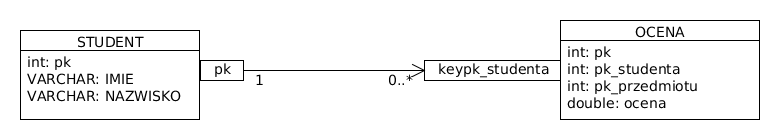
\includegraphics[width=1.000\linewidth]{downloads/wyklad1/data/relacja.png}}
\caption{Przykład schematu relacyjnego}
\end{figure}

Ważne cechy schematu relacyjnego:
%
\begin{itemize}

\item Dane są przechowywane tylko w wierszach tabel.

\item Tabele mają kolumny o ustalonym typie.

\item Na poszczególne wiersze nałożone mogą być pewne ograniczenia.

\item System musi być przygotowany do repreezentowania \textquotedbl{}braku informacji\textquotedbl{}

\end{itemize}

Opcjonalnie możecie się~zapoznać z tym dokumentem: \url{http://en.wikipedia.org/w/index.php?title=Codd\%27s_12_rules&oldid=574873395}.

Informacje o strukturze danych w bazie nazywamy
schematem (z ang. database schema).


\subsection{Wartość NULL%
  \label{wartosc-null}%
}

Wartość \texttt{NULL} reprezentuje informację o tym, że dana wartość jest niedostępna.
Jeśli w kolumnie 'ocena' zawarta jest wartość \texttt{NULL} oznacza to, że system nie posiada
informacji o danej ocenie.

Wprowadzenie wartości \texttt{NULL} jest ważne ponieważ pozwala ona jasno i jednoznacznie
powiedzieć: tej informacji nie mamy oraz żadna poprawna wartość w żadnej kolumnie
nigdy nie będzie równa NULL. Bez wartości \texttt{NULL} musielibyśmy uznać, że np. ocena
\texttt{-1} oznacza, że dany ocena nie jest dostępna, co jest mniej oczywiste.


\subsection{Ograniczenia w bazie danych%
  \label{ograniczenia-w-bazie-danych}%
}

Systemy relacyjne pozwalają nakładać na schemat pewne ograniczenia albo inaczej
więzy (\emph{z ang.} constraints) przykłady klasy ograniczeń zawartych w przykładzie:

klucz główny \emph{z ang.} primary key
%
\begin{quote}

Kolumna \texttt{id} tabeli student jest unikalna (dwóm wierszom nie może być
przypisana taka sama wartość w tej kolumnie) oraz nie może przyjmować
wartości pustej. Klucz główny jednoznacznie definiuje dany wiersz w tabeli.

\end{quote}

nie pustość \emph{z ang.} non null
%
\begin{quote}

Kolumny \texttt{imie} oraz \texttt{nazwisko} nie mogą zawierać wartości pustej \texttt{NULL}

\end{quote}

sprawdzenie \emph{z ang.} check constraint
%
\begin{quote}

Check constraint pozwala wymusić, by dany wiersz spełniał zadane wyrażenie
logiczne. W kolumnie ocena są wartości od 2 do 5.

\end{quote}

klucz obcy \emph{z ang.} foreign key
%
\begin{quote}

Jeśli w tabeli \texttt{ocena} w kolumnie \texttt{pk\_studenta} będzie
wartość X, to istnieje student o \texttt{id} równym X.

To ograniczenie pozwala definiować zależności między tabelami mówimy, że
ocena A jest oceną studenta B jeśli w kolumnie 'pk\_studenta' jest
identyfikator studenta A.

\end{quote}


\subsection{Spójność danych%
  \label{spojnosc-danych}%
}

Wymuszanie podanych w poprzednim paragrafie ograniczeń mogłoby być
nietrywialne, jednak to silnik bazy danych wymusza je za nas.

To jest pierwsza ważna cecha baz danych: programista definiuje
schemat a baza danych go wymusza.


\section{Baza danych postgresql%
  \label{baza-danych-postgresql}%
}

Będziemy korzystać z bazy danych PostgreSQL. Baza ta jest najbardziej
zaawansowaną opensource bazą danych na rynku oraz jest dość zgodna
ze standardem SQL.


\subsection{Narzędzia administracyjne bazy danych%
  \label{narzedzia-administracyjne-bazy-danych}%
}


\subsubsection{Polecenie konsolowe \texttt{psql}%
  \label{polecenie-konsolowe-psql}%
}

Polecenie to pozwala na interakcje z bazą danych za pomocą
konsoli. Zasadniczo ma ono wszystkie możliwości klientów
graficznych.

Podstawowa składania polecenia to:

\begin{verbatim}
psql [baza danych]
\end{verbatim}

W tym trybie psql przyjmie polecenia ze standardowego wejścia
w trybie interaktywnym.

Możemy też zmusić go do przetworzenia pliku wejściowego:

\begin{verbatim}
psql -f [plik] [baza danych]
\end{verbatim}

Pełny opis polecenia: \url{http://www.postgresql.org/docs/9.2/static/app-psql.html}.


\subsubsection{Interfejs graficzny PGADMIN%
  \label{interfejs-graficzny-pgadmin}%
}

Bardzo potężne narzędzie, jest natomiast dość proste w obsłudze.
Jedynym problemem, jaki mogą Państwo mieć jest to, by w łączeniu
do lokalnego komputera pole host zostawić puste.
Słowem  konfiguracja serwera powinna być taka:

\begin{figure}
\noindent\makebox[\textwidth][c]{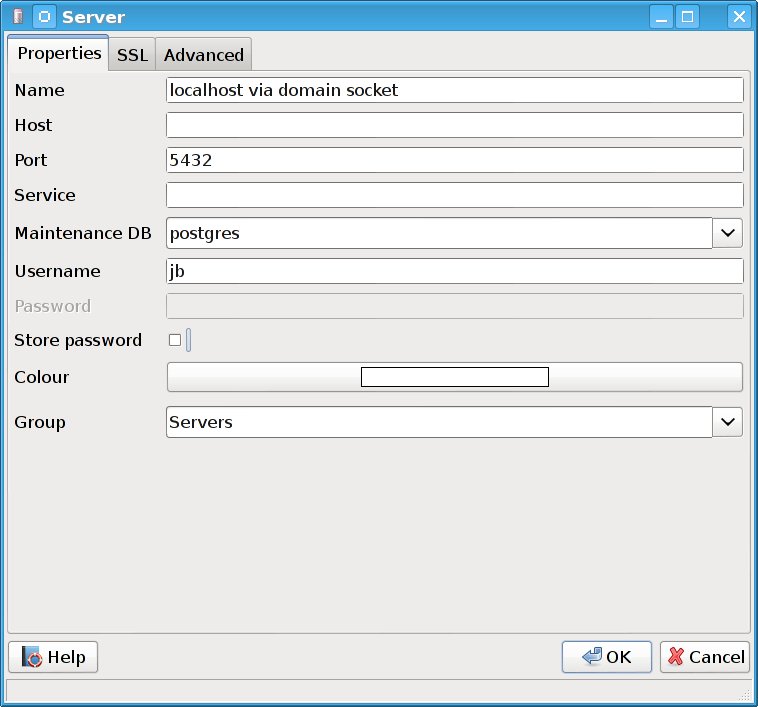
\includegraphics[width=1.000\linewidth]{downloads/wyklad1/data/postgres-add-database.png}}
\caption{Poprawna konfiguracja postgresql}
\end{figure}


\section{Wybieranie danych%
  \label{wybieranie-danych}%
}

Do pobierania danych z bazy dancyh służy polecenie \texttt{SELECT}

\DUadmonition[note]{
\DUtitle[note]{Note}

Proszę nie myśleć o poleceniu \texttt{SELECT},
jako o metodzie na wybieranie danych, ale raczej jako o metodzie
opisywania danych, które chcemy pobrać.

Opis ten jest oderwany
od tego w jaki sposób to zapytanie należy wykonać -{}-{}-
o to martwi się serwer baz danych.
}


\subsection{Składnia polecenia SELECT%
  \label{skladnia-polecenia-select}%
}

W najprostszej wersji polecenie to ma taką postać:

\begin{verbatim}
SELECT * FROM tabela;
\end{verbatim}

\attachfile{downloads/wyklad1/data/selectstar.html}{Wynik zapytania}

Znaczy ono: zbiór danych, który chce pobrać zawiera dane
ze wszystkich kolumn i wszystkich wierszy tabeli.

Na pierwszych zajęciach będziemy pracowali na takiej tabeli:

\begin{figure}
\noindent\makebox[\textwidth][c]{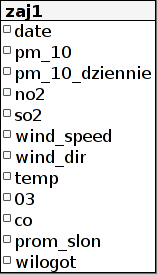
\includegraphics[width=0.300\linewidth]{downloads/wyklad1/data/zaj1-schema.png}}
\caption{Schemat do pierwszych zajęć}
\end{figure}

Tabela ta zawiera parametry pogodowe i poziomy zanieczyszczeń
stacji Warszawa Ursynów.

Ważne informacje o schemacie:
%
\begin{itemize}

\item Kolumna \texttt{date} zawiera chwilę zebrania pomiaru

\item Kolumna \texttt{pm\_10} zawiera poziom pyłu zawieszonego $PM_{10}$.

\item kolumna \texttt{wind\_speed} zawiera kierunek wiatru (w stopniach!)

\end{itemize}


\subsection{Klauzula WHERE%
  \label{klauzula-where}%
}

Do ograniczania zakresu wybieranych rzędów danych służy klauzula \texttt{WHERE},
Powiedzmy, że chcemy wybrać dane ze stycznia 2012 roku.

\begin{verbatim}
SELECT * FROM zaj1 WHERE date
  BETWEEN '2012-01-01' AND '2012-01-31';
\end{verbatim}

\attachfile{downloads/wyklad1/data/selectwhere.html}{Wyniki zapytania}

\DUadmonition[note]{
\DUtitle[note]{Note}

Poza klauzulą where mamy tutaj kilka cech języka postgresql. Za pomocą
znaków \texttt{'} oznaczamy stałe określające ciągi znaków.

\emph{Poboczna uwaga}: to że
podałem datę jako ciąg znaków, nie oznacza, że w ten sposób daty są
przechowywane w bazie danych (jest to wydajniejszy format), po prostu
postgres umie rzutować ciągi znaków w dobrym formacie na datę.
}

Klauzula \texttt{WHERE} przyjmuje dowolne wyrażenie logiczne, w tym zapytaniu wybieramy
dane ze stycznia w dniach, w których jednocześnie przekroczono poziomy
$PM_{10}$ oraz $NO_2$:

\begin{verbatim}
SELECT * FROM zaj1
    WHERE date BETWEEN '2012-01-01'
        AND '2012-01-31' AND ( pm_10 > 50 or no_2 > 200);
\end{verbatim}

\attachfile{downloads/wyklad1/data/selectwhere_expre.html}{Wyniki zapytania}

Dodatkowe informacje:
%
\begin{itemize}

\item \href{https://www.google.pl/?q=postgresql\%209.2\%20logical\%20operators\#q=postgresql+9.2+logical+operators}{Operatory logiczne w PostgreSQL}

\item \href{https://www.google.pl/?q=postgresql\%209.2\%20comparision\%20operators\#q=postgresql+9.2+comparision+operators}{Operatory porównania w PostgresQL}

\end{itemize}


\subsection{Wybieranie kolumn%
  \label{wybieranie-kolumn}%
}

Możemy określać, jakie kolumny zbioru wynikowego nas interesują,
na przykład, żeby wybrać datę i kierunek wiatru możemy napisać,
w takim wypadku po słowie \texttt{SELECT} pojawia się lista wyrażeń, które
określają poszczególne kolumny wybranego zbioru danych:

\begin{verbatim}
SELECT date, wind_dir FROM zaj1;
\end{verbatim}

\attachfile{downloads/wyklad1/data/selectcolumn.html}{Wynik zapytania}

Nie musimy wybierać kolumn tabeli, możemy wybrać dowolne wyrażenia, które
operują (lub nie) na danych z poszczególnych kolumn.

\begin{verbatim}
SELECT date, radians(wind_dir) FROM zaj1;
\end{verbatim}

\attachfile{downloads/wyklad1/data/selectradians.html}{Wynik zapytania}

Wyrażenia wybierane mogą być całkiem dowolne:

\begin{verbatim}
SELECT 6/2*(1+2) FROM zaj1;
\end{verbatim}

\attachfile{downloads/wyklad1/data/select-zagadka.html}{Wynik zapytania}

Możemy też wykonywać zapytania wybierające dane z wielu kolumn:

\begin{verbatim}
SELECT no_2 + pm_10 AS nonsens FROM zaj1;
\end{verbatim}

\attachfile{downloads/wyklad1/data/select-nonsense.html}{Wynik zapytania}

W tym zapytaniu użyto również klauzuli \texttt{AS}, która pozwala
wyrażeniu (lub kolumnie) nadać określoną nazwę w zbiorze wynikowym.

Dodatkowe informacje:
%
\begin{itemize}

\item \href{https://www.google.pl/?q=postgresql\%209.2\%20mathematical\%20functions\#q=postgresql+9.2+mathematical+functions}{Matematyczne funkcje w postgresql}

\end{itemize}


\subsection{Sortowanie danych%
  \label{sortowanie-danych}%
}

Domyślnie dane dane wybierane z zestawu danych, nie są sortowane,
albo inaczej: \emph{są wybierane w takiej kolejności w jakiej serwerowi wygodnie}
Przy prostych zapytaniach jest to kolejność, w których dane leżą na dysku, a
ponieważ do tej tabeli dane były dodawane w kolejności dat, w takiej kolejności
pojawiły się na dysku i tak są wybierane.

By wymusić sortowanie wyników względem jakiejś kolumny używamy klauzuli
order by:

\begin{verbatim}
SELECT * FROM zaj1 ORDER BY date desc;
\end{verbatim}

\attachfile{downloads/wyklad1/data/selectorder.html}{Wyniki zapytania}, proszę porównać z
\attachfile{downloads/wyklad1/data/selectstar.html}{tym samym zapytaniem bez klauzuli order by}

Słowo \texttt{desc} (skrót ot \emph{descending}) oznacza kierunek sortowania od wartości największej do najmniejszej.
Przy uznaniu co oznacza wartość \emph{największa} i \emph{najmniejsza} można kierować
się intuicją, jedyny problem jest z \href{https://www.google.com/search?q=postgresql+string+collation}{sortowaniem i porównywaniem ciągów znaków}.  By posortować
dane od wartości najmniejszej do największej należałoby użyć \texttt{asc} (\emph{ascending}).
Domyślnie (bez podania \texttt{desc} i \texttt{asc}) dane są sortowane od najmniejszej do
największej.

Proszę poprzednie zapytanie z:

\begin{verbatim}
SELECT date, wind_dir, pm_10 FROM zaj1
  ORDER by wind_dir;
\end{verbatim}

\attachfile{downloads/wyklad1/data/selectordermany-compare.html}{Wynik zapytania}

Możemy też sortować względem wyrażenia:

\begin{verbatim}
SELECT date, sin(radians(wind_dir)) FROM zaj1
  ORDER by sin(radians(wind_dir));
\end{verbatim}

\attachfile{downloads/wyklad1/data/selectorderexpression.html}{Wynik zapytania}


\section{Funkcje agregujące (opcjonalne -{}- nie będzie na zajęciach)%
  \label{funkcje-agregujace-opcjonalne-nie-bedzie-na-zajeciach}%
}

Ilość analiz jakie możemy zrobić za pomocą operacji na pojedyńczych wierszach
jest ograniczona.

Powiedzmy że chcemy poznać średni poziom zanieczyczeń dla całego zestawu
danych:

\begin{verbatim}
SELECT AVG(pm_10), AVG(NO_2) FROM zaj1;
\end{verbatim}

\attachfile{downloads/wyklad1/data/selectavg.html}{Wynik zapytania}.

Proszę zauważyć że klauzula \texttt{AVG} oraz inne funkcje agregujące
(\emph{z. ang} aggregate functions) całkiem zmienia nam wybrany zestaw danych!
W tym wypadku powoduje, że w zestawie wyikowym mamy jeden wiersz.

By wybrać średni poziom z jakiegoś okresu czasu należałoby
dodać klauzulę \texttt{where}

\begin{verbatim}
SELECT AVG(pm_10) FROM zaj1
  WHERE date BETWEEN '2012-01-01' AND '2012-01-31';
\end{verbatim}

\attachfile{downloads/wyklad1/data/selectavg-where.html}{Wynik zapytania}

Przykłady funkcji agregujących:

\texttt{COUNT}
%
\begin{quote}

Zwraca ilość wierszy w zestawie danych

\end{quote}

\texttt{STDDEV}
%
\begin{quote}

Zwraca odchylenie standardowe

\end{quote}

\texttt{AVG}
%
\begin{quote}

Zwraca średnią

\end{quote}

\texttt{MAX}
%
\begin{quote}

Zwraca największą wartość z zestawu danych

\end{quote}

\href{https://www.google.pl/?q=postgresql\%209.2\%20aggregate\%20functions}{Więcej funkcji agregujących}


\subsection{Klauzula \texttt{GROUP BY}%
  \label{klauzula-group-by}%
}

Wybranie średniej całego zestawu danych też ma ograniczoną
przydatność, by wykonać funkcje agregujące na pewnych podzbiorach
danych należy użyć klauzuli \texttt{GROUP BY}.

Klauzula ta przyjmuje kolumnę bądź wyrażenie oraz powoduje podział
zbioru danych na podgrupy, dla których wyrażenie w \texttt{group by} przyjmuje
taką samą wartśsć oraz wyznaczenie funkcji agregujących dla tych
podgrup oddzielnie.

\begin{verbatim}
SELECT AVG(wind_speed), pm_10 > 50 as przekroczenie
FROM zaj1 GROUP BY pm_10 > 50;
\end{verbatim}

\attachfile{downloads/wyklad1/data/selectavg-group-by.html}{Wynik zapytania}

W tym wypadk dzielimy zbiór danych na dwa podzbiory: w pierwszym
nastąpiło przekroczenie dopuszczalnego dziennego poziomu pyłu zawieszonego
$PM_{10}$, w drugim przekroczenia nie było.

\begin{verbatim}
SELECT AVG(wind_speed), wind_dir, COUNT(*)
FROM zaj1 GROUP BY wind_dir ORDER BY wind_dir;
\end{verbatim}

\attachfile{downloads/wyklad1/data/selectavg-group-by-2.html}{Wynik zapytania}

Teraz grup mamy 360 (tyle ile jest różnych wartości kierunku wiatru).

Gdy w wyrażeniu pojawia się klauzula \texttt{GROUP BY} znacznie ogranicza
się to, co możemy podać po klauzuli \texttt{SELECT}, mianowicie możemy podać:
\newcounter{listcnt0}
\begin{list}{\arabic{listcnt0}.}
{
\usecounter{listcnt0}
\setlength{\rightmargin}{\leftmargin}
}

\item Wyrażenie zawierające wynik działania funkcji agregujących na
\emph{dowolnych} kolumnach

\item Wyrażenie zawierające wyrażenie przekopiowane z klauli \texttt{GROUP BY}
\end{list}

Przykładowo w zapytaniu z klauzulą \texttt{GROUP BY sin(radians(wind\_speed))}
może pojawić się:
%
\begin{itemize}

\item Wyrażenie \texttt{AVG(pm\_10)} (zasada 1)

\item Wyrażenie \texttt{sin(radians(wind\_speed))} (zasada 2)

\end{itemize}

Nie może natomiast pojawić się:
%
\begin{itemize}

\item Wyrażenie \texttt{pm\_10}

\item Wyrażenie \texttt{wind\_speed} (mimo że kolumna \texttt{wind\_speed} była użyta w
grupowaniu)

\end{itemize}

Takie ograniczenie ma bardzo proste uzasadnienie: po zgrupowaniu względem
jakiegoś wyrażenia każdemu wierszowi tworzonego zbioru wynikowego
przypisane jest wiele wierszy z tabeli (wszystkie, dla których wyrażenie \texttt{GROUP BY}
przyjmuje jedną wartość), a baza danych 'nie bardzo wie', którą z tych wartości
wybrać. My możemy: albo dać bazie danych przepis o tym, jak z tego zbioru danych
stworzyć jedną wartość do wyświetlenia (przepisem tym jest funkcja agregująca),
albo musimy wybrać wyrażenie z klauzuli \texttt{GROUP BY}, ponieważ dla każdego
wiersza w zbiorze danych z definicji wyrażenie to musi dać tą samą wartość.

Proszę zastanowić się dlaczego takie zapytanie jest poprawne:

\begin{verbatim}
SELECT AVG(pm_10), AVG(NO_2), sin(radians(wind_speed))
  FROM zaj1 GROUP BY wind_speed;
\end{verbatim}

\attachfile{downloads/wyklad1/data/select-group-by-ciekawostka-1.html}{Wynik zapytania:}

A takie nie:

\begin{verbatim}
SELECT AVG(pm_10), AVG(NO_2), wind_speed
  FROM zaj1
  GROUP BY sin(radians(wind_speed));
\end{verbatim}


\subsection{Dodatnowe przykłady:%
  \label{dodatnowe-przyklady}%
}

Powiedzmy, że chcemy wyznaczyć dzienne średnie poziomy pyłu zawieszonego
$PM_{10}$, by tego użyć musimy użyć funkcji \texttt{date\_trunc}, powoduje ona
obcięcie wartości przechowującej czas do wyznaczonej dokładności.

Przykładowo nastpujące dwa zapytania zwracają \texttt{true}:

\begin{verbatim}
SELECT date_trunc('day', '2012-01-07 11:11'::date) = '2012-01-07';
SELECT date_trunc('month', '2012-01-07 11:11'::date) = '2012-01-01';
\end{verbatim}


\subsection{Klauzula \texttt{HAVING}%
  \label{klauzula-having}%
}

Klauzula ta działa jak klauzula where, ale pozwala filtrować
względem agregowanych wartości, na przykład by wybrać dni,
dla których poziom \texttt{PM\_10} jest większy niż norma
należy wykonać zapytanie:

\begin{verbatim}
SELECT AVG(pm_10), date_trunc('day', date)
  FROM zaj1
  GROUP BY date_trunc('day', date)
  HAVING AVG(pm_10) > 50 ORDER BY date_trunc('day', date);
\end{verbatim}

\attachfile{downloads/wyklad1/data/selectavg-group-by-having.html}{Wynik zapytania}

Wyrażenie having, pozwala filtrować zbiór danych pod względem wyrażeń
zawierających funkcje agregujące.

Proszę zastanowić się czym różni się klauzula \texttt{WHERE} od klauzuli \texttt{HAVING}.

\end{document}
